\section{Applications}

\begin{frame}{2-D shape interpolation}
    \vspace{-1.2em}
    \begin{figure}
        \centering
        \captionsetup{font=scriptsize}
        \begin{minipage}[t]{0.08\linewidth}
            \vspace{0pt}
            \centering
            
\includegraphics[width=\textwidth]{png/kun-chicken/color0.png}
        \end{minipage}
        \hfill
        \begin{minipage}[t]{0.08\linewidth}
            \vspace{0pt}
            \centering
            
\includegraphics[width=\textwidth]{png/kun-chicken/color1.png}
        \end{minipage}
        \hfill
        \begin{minipage}[t]{0.08\linewidth}
            \vspace{0pt}
            \centering
            
\includegraphics[width=\textwidth]{png/kun-chicken/color2.png}
        \end{minipage}
        \hfill
        \begin{minipage}[t]{0.08\linewidth}
            \vspace{0pt}
            \centering
            
\includegraphics[width=\textwidth]{png/kun-chicken/color3.png}
        \end{minipage}
        \hfill
        \begin{minipage}[t]{0.08\linewidth}
            \vspace{0pt}
            \centering
            
\includegraphics[width=\textwidth]{png/kun-chicken/color4.png}
        \end{minipage}
        \hfill
        \begin{minipage}[t]{0.08\linewidth}
            \vspace{0pt}
            \centering
            
\includegraphics[width=\textwidth]{png/kun-chicken/color5.png}
        \end{minipage}
        \hfill
        \begin{minipage}[t]{0.08\linewidth}
            \vspace{0pt}
            \centering
            
\includegraphics[width=\textwidth]{png/kun-chicken/color6.png}
        \end{minipage}
        \hfill
        \begin{minipage}[t]{0.08\linewidth}
            \vspace{0pt}
            \centering
            
\includegraphics[width=\textwidth]{png/kun-chicken/color7.png}
        \end{minipage}
        \hfill
        \begin{minipage}[t]{0.08\linewidth}
            \vspace{0pt}
            \centering
            
\includegraphics[width=\textwidth]{png/kun-chicken/color8.png}
        \end{minipage}
        \hfill
        \begin{minipage}[t]{0.08\linewidth}
            \vspace{0pt}
            \centering
            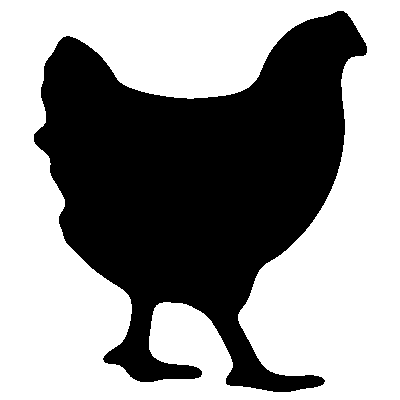
\includegraphics[width=\textwidth]{png/kun-chicken/color9.png}
        \end{minipage}

        \vspace{.3em}
        \begin{minipage}[t]{0.08\linewidth}
            \vspace{0pt}
            \centering
            
\includegraphics[width=\textwidth]{png/kun-chicken/shape-1-1.png}
        \end{minipage}
        \hfill
        \begin{minipage}[t]{0.08\linewidth}
            \vspace{0pt}
            \centering
            
\includegraphics[width=\textwidth]{png/kun-chicken/shape-1-2.png}
        \end{minipage}
        \hfill
        \begin{minipage}[t]{0.08\linewidth}
            \vspace{0pt}
            \centering
            
\includegraphics[width=\textwidth]{png/kun-chicken/shape-1-3.png}
        \end{minipage}
        \hfill
        \begin{minipage}[t]{0.08\linewidth}
            \vspace{0pt}
            \centering
            
\includegraphics[width=\textwidth]{png/kun-chicken/shape-1-4.png}
        \end{minipage}
        \hfill
        \begin{minipage}[t]{0.08\linewidth}
            \vspace{0pt}
            \centering
            
\includegraphics[width=\textwidth]{png/kun-chicken/shape-1-5.png}
        \end{minipage}
        \hfill
        \begin{minipage}[t]{0.08\linewidth}
            \vspace{0pt}
            \centering
            
\includegraphics[width=\textwidth]{png/kun-chicken/shape-1-6.png}
        \end{minipage}
        \hfill
        \begin{minipage}[t]{0.08\linewidth}
            \vspace{0pt}
            \centering
            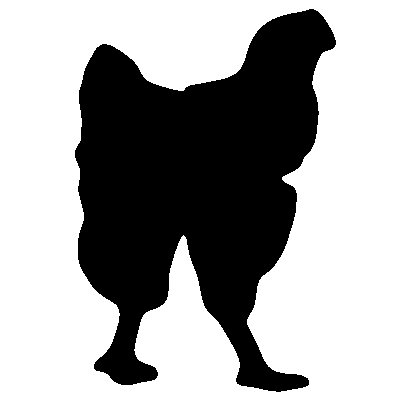
\includegraphics[width=\textwidth]{png/kun-chicken/shape-1-7.png}
        \end{minipage}
        \hfill
        \begin{minipage}[t]{0.08\linewidth}
            \vspace{0pt}
            \centering
            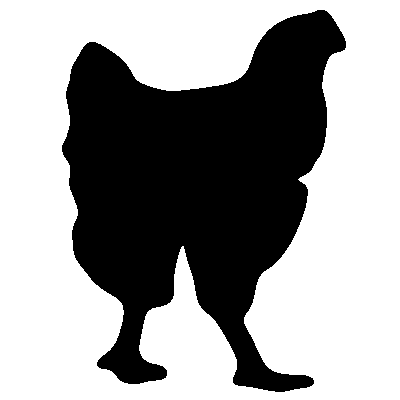
\includegraphics[width=\textwidth]{png/kun-chicken/shape-1-8.png}
        \end{minipage}
        \hfill
        \begin{minipage}[t]{0.08\linewidth}
            \vspace{0pt}
            \centering
            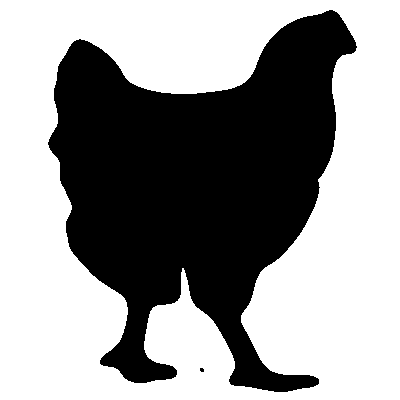
\includegraphics[width=\textwidth]{png/kun-chicken/shape-1-9.png}
        \end{minipage}
        \hfill
        \begin{minipage}[t]{0.08\linewidth}
            \vspace{0pt}
            \centering
            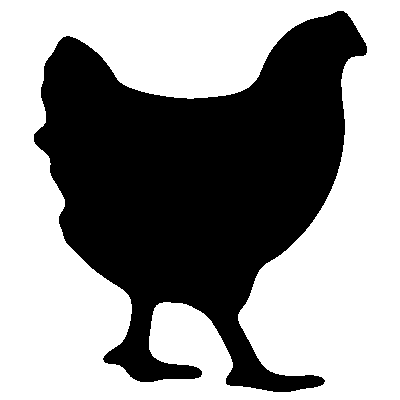
\includegraphics[width=\textwidth]{png/kun-chicken/shape-1-10.png}
        \end{minipage}
        
        \caption{From Kunkun to chicken. Top: color interpolation. Bottom: shape interpolation.}
    \end{figure}

    \vspace{-1.2em}
    \begin{figure}
        \centering
        \captionsetup{font=scriptsize}
        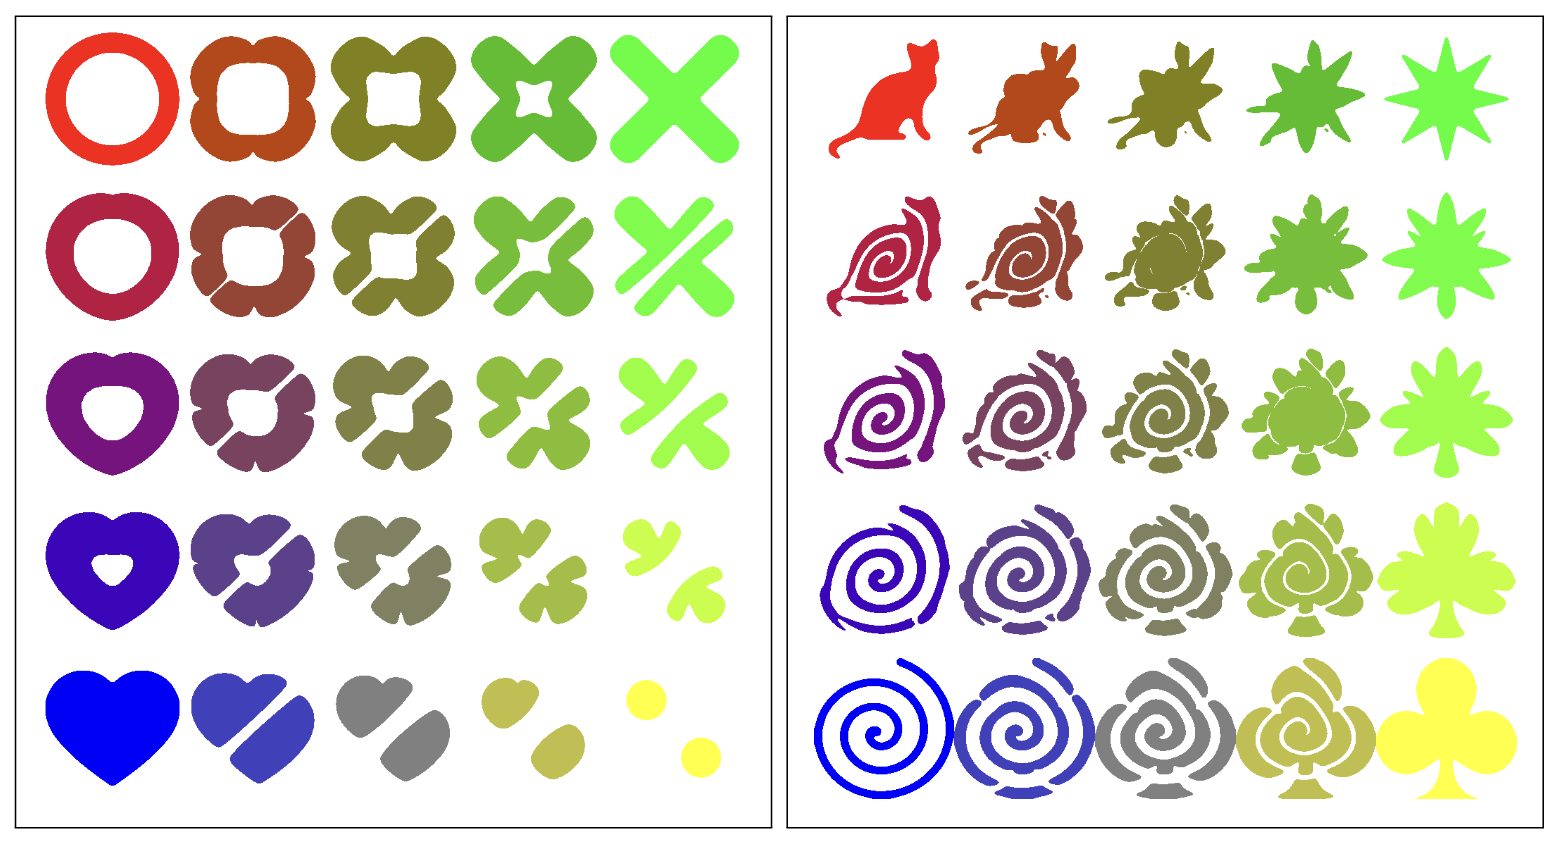
\includegraphics[width=0.6\textwidth]{png/2DShapeInterpolation.png}
        \caption{Barycenter of four shapes\footfullcite{peyre2019computational}.}
    \end{figure}
\end{frame}

\begin{frame}{Color transfer}
    \footnotesize
    Compute a transformation $T$ such that 
    \begin{equation}
        I_Z(x) = T (I_X(x)),\quad \text{for all pixel}\;x,
    \end{equation}
    where the new color distribution $\mu_Z$ is close or equal to $\mu_Y$.
    \begin{figure}
        \centering
        \captionsetup{font=scriptsize}
        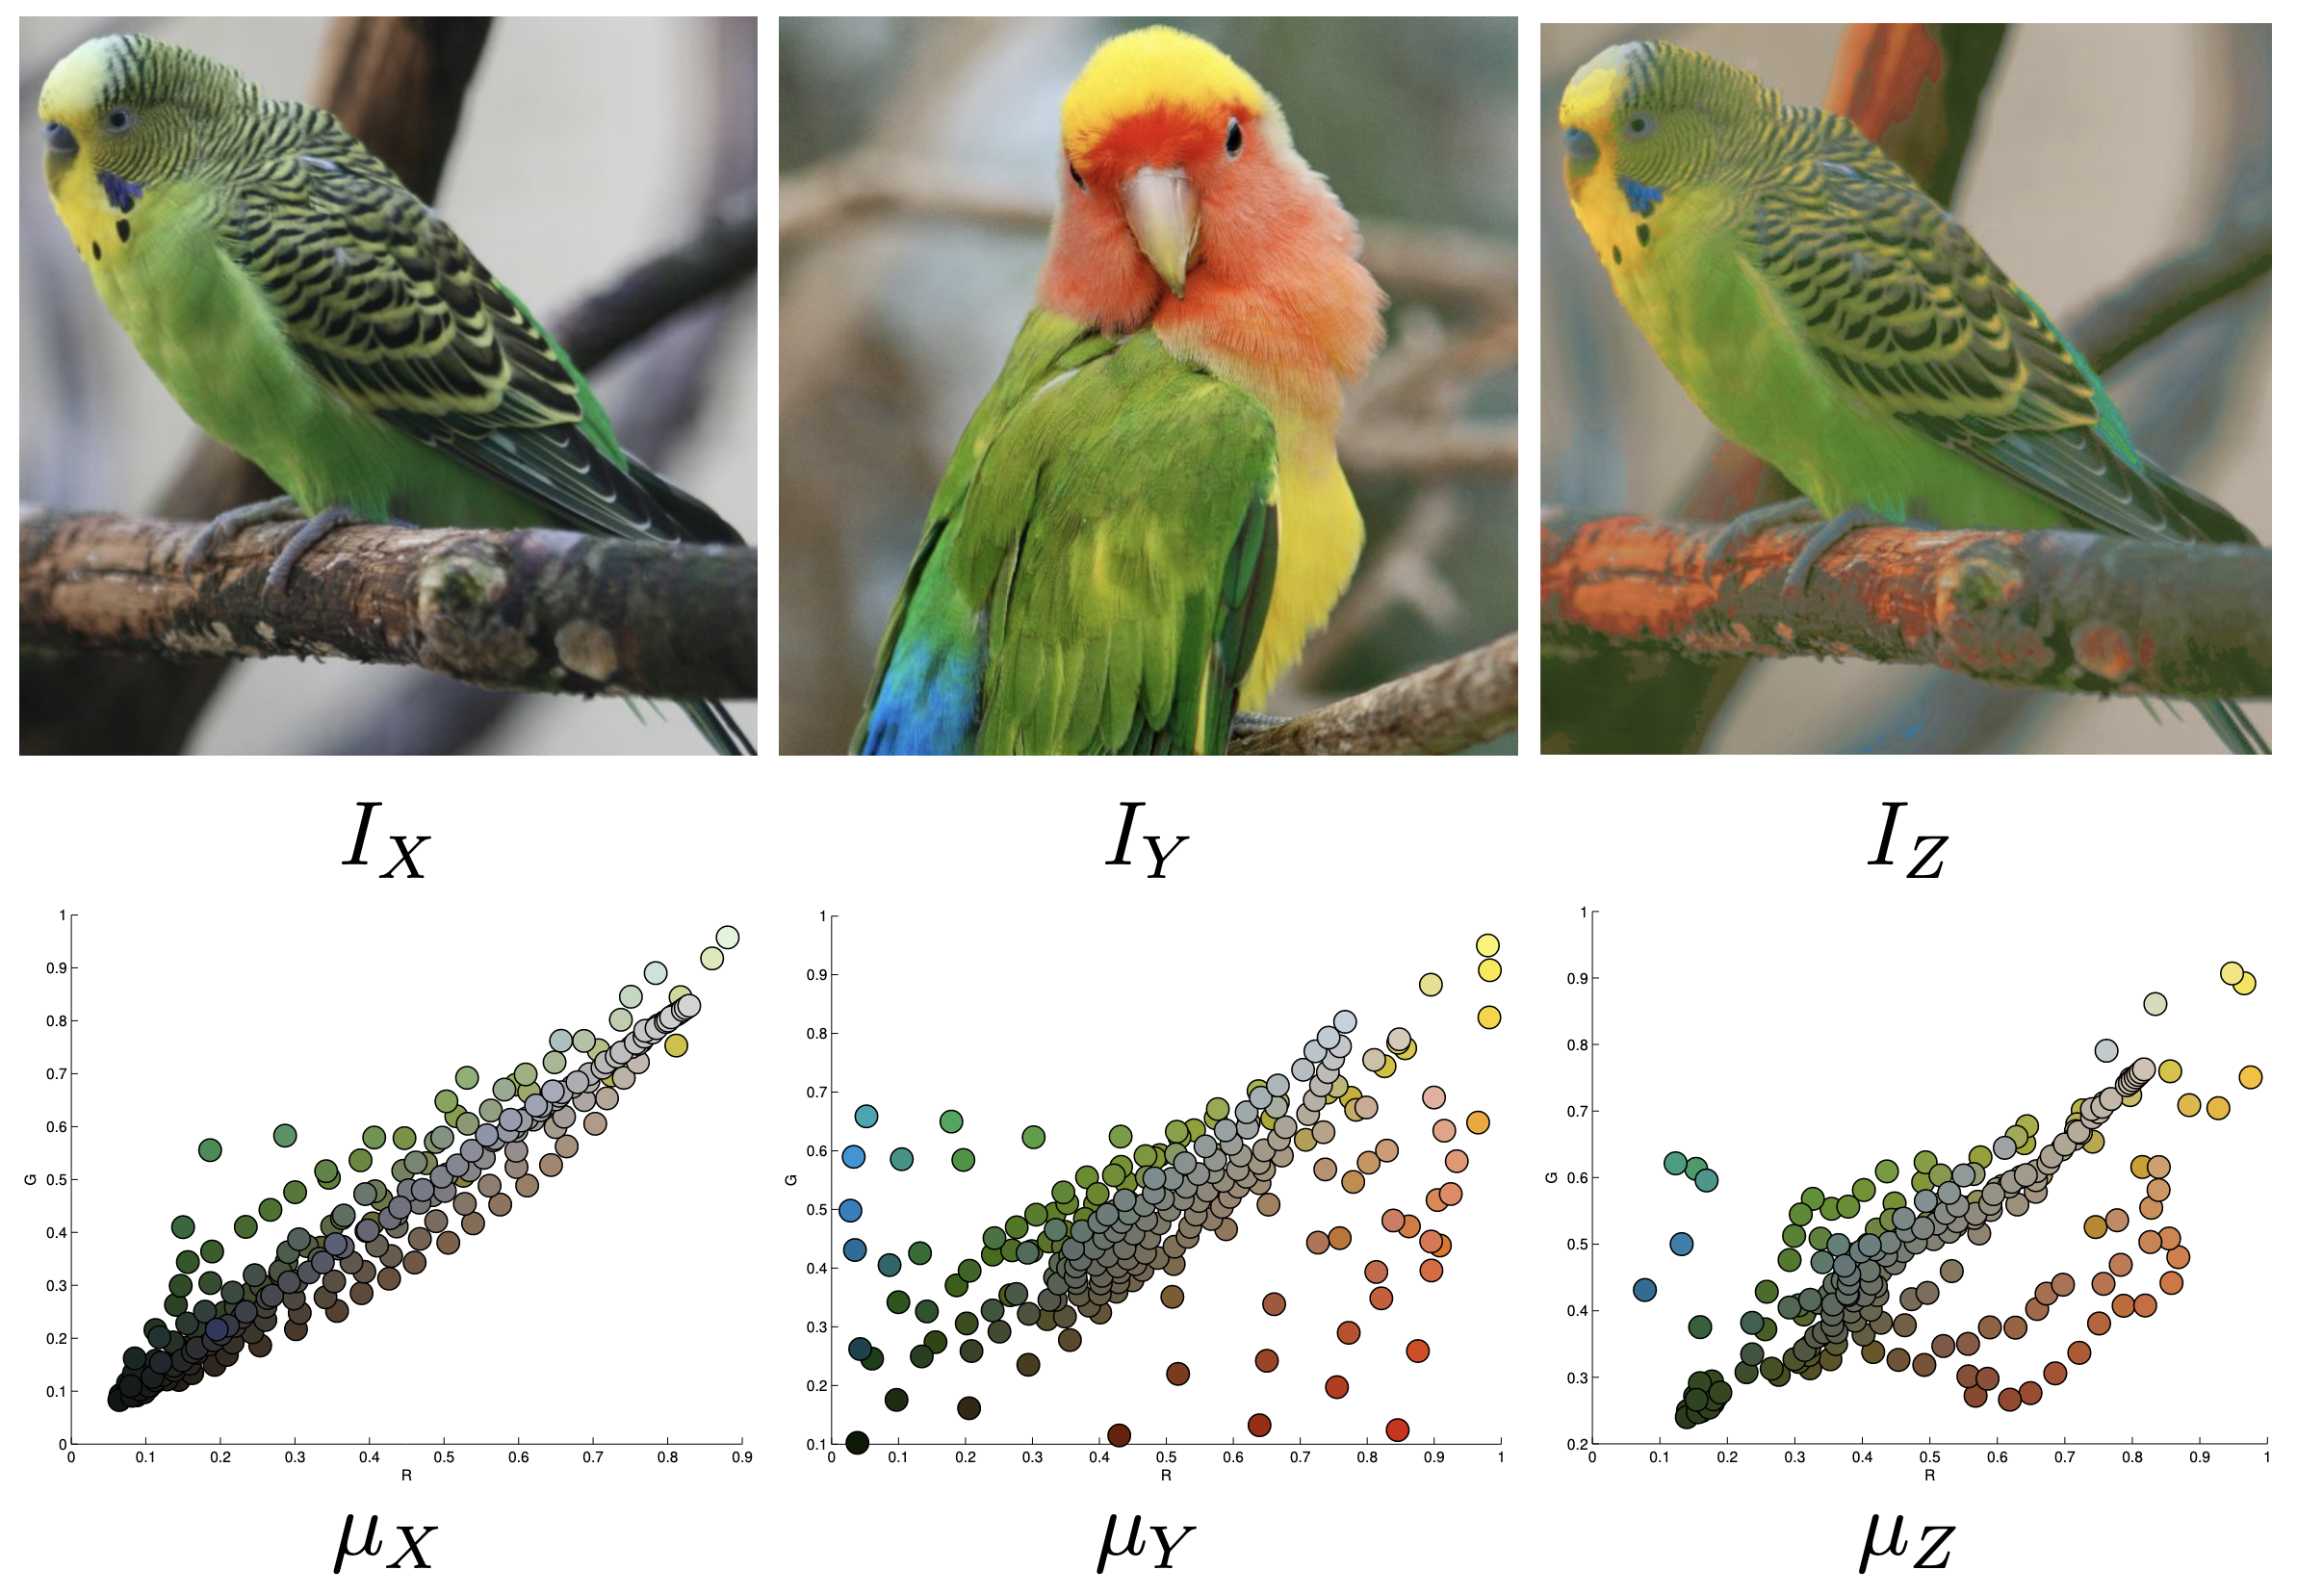
\includegraphics[width=0.65\textwidth]{png/color-transfer.png}
        \caption{Example of color transfer\footfullcite{papadakis2015optimal}. 
        The second row representes RGB color distributions using the 2-D projection of every pixel in the RG plane}
    \end{figure}
\end{frame}

\begin{frame}{Color transfer}
    \footnotesize
    \begin{figure}
        \centering
        \captionsetup{font=scriptsize}
        \begin{minipage}[b]{0.45\linewidth}
            \vspace{0pt}
            \centering
            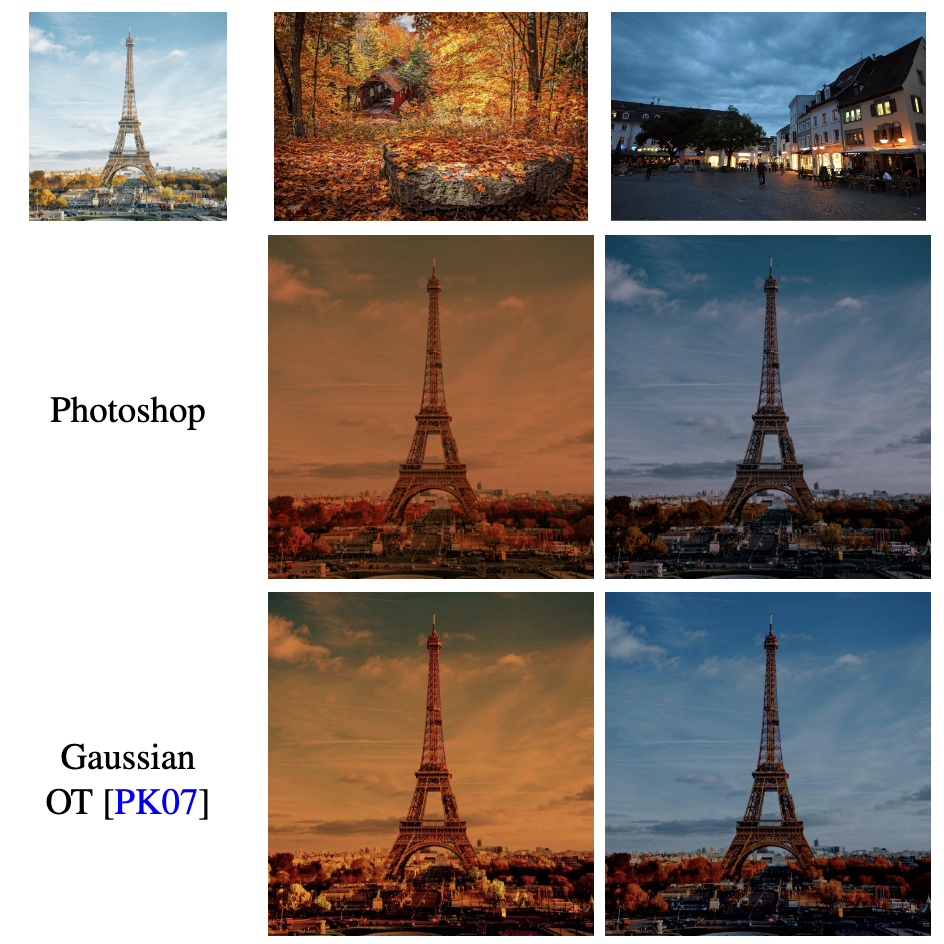
\includegraphics[width=\textwidth]{png/tower-ctrans.png}
        \end{minipage}
        \hfill
        \begin{minipage}[b]{0.45\linewidth}
            \vspace{0pt}
            \centering
            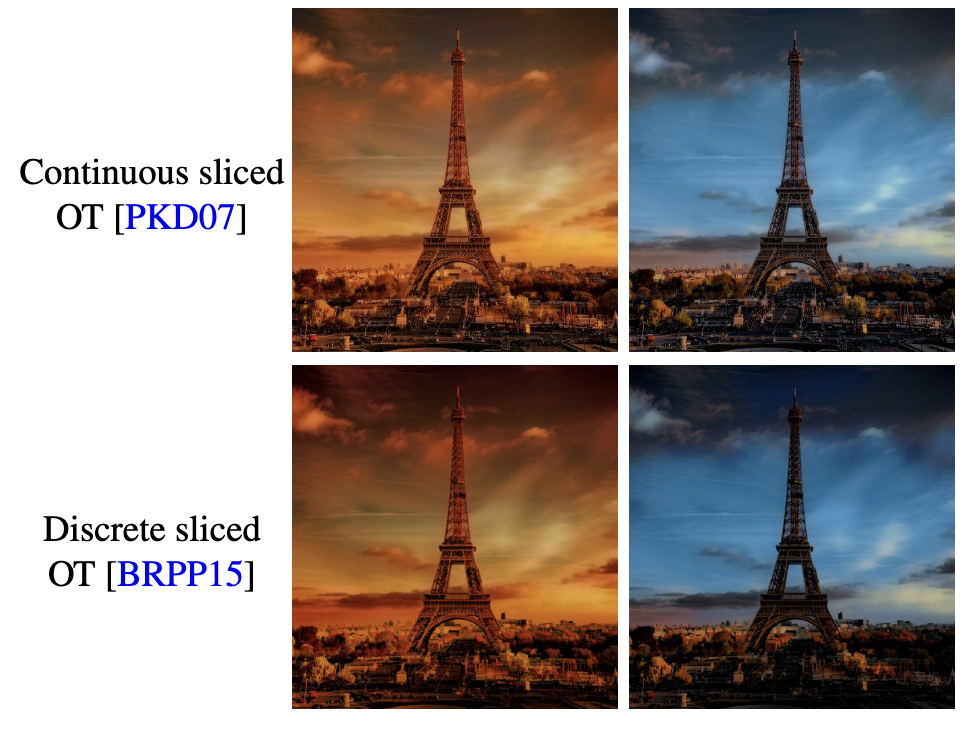
\includegraphics[width=\textwidth]{png/tower-ctrans2.png}
        \end{minipage}
        \caption{Another example of color transfer\footfullcite{bonneel2023survey}.}
    \end{figure}
\end{frame}

\begin{frame}{Fluid dynamics}
    \footnotesize
    \begin{figure}
        \centering
        \captionsetup{font=scriptsize}
        \centering
        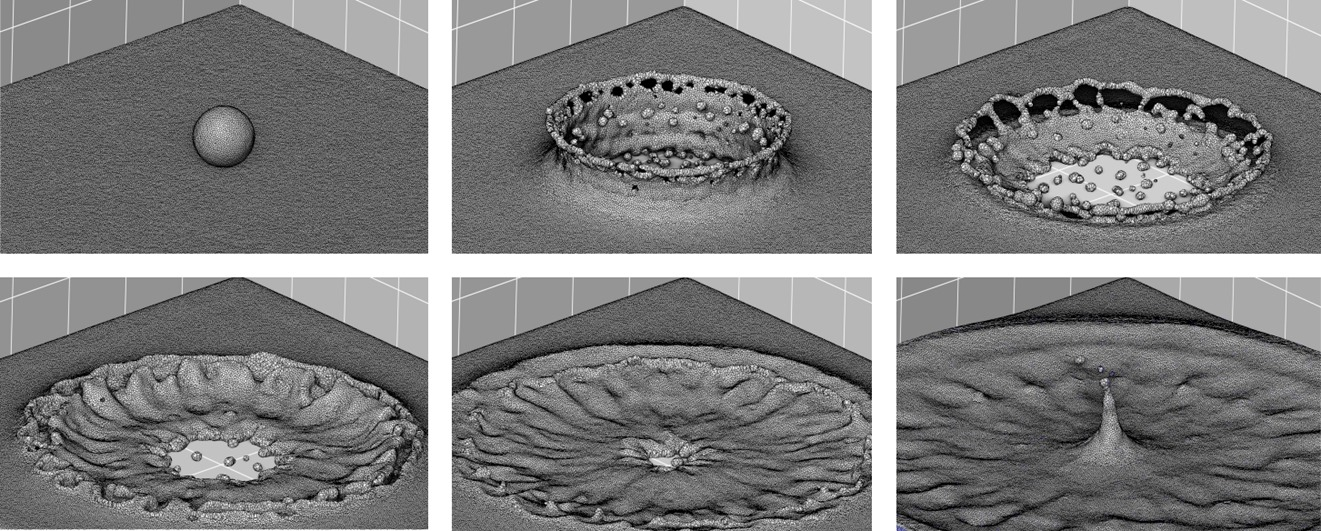
\includegraphics[width=\textwidth]{png/cfd.jpg}
        \caption{Simulation of the free boundary problem using partial OT\footfullcite{levy2022partial}.}
    \end{figure}
\end{frame}

\begin{frame}{Area-preservation mapping\footfullcite{gxfot2013}}
    \footnotesize
    \vspace{-1.2em}
    \begin{figure}
        \centering
        \captionsetup{font=scriptsize}
        \begin{minipage}[c]{0.45\linewidth}
            \vspace{0pt}
            \centering
            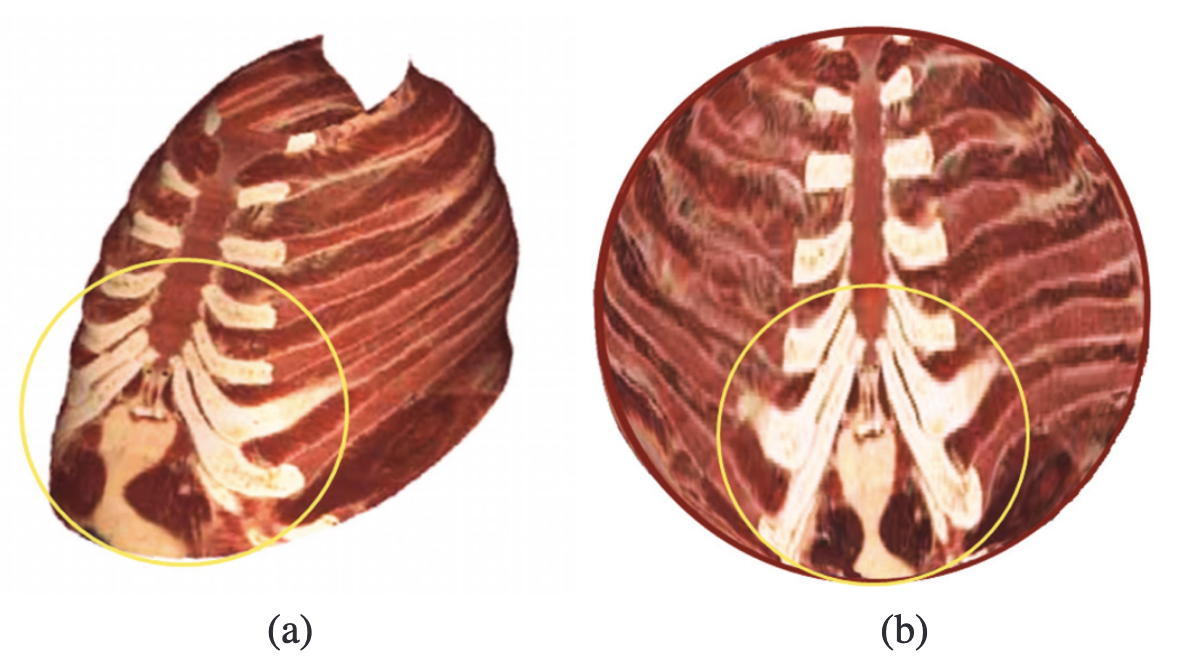
\includegraphics[width=\textwidth]{png/bones.png}
            \caption{Surface flattening of a chest model using 
            area-preservation mapping for direct display and accurate measurement. 
            The yellow circles highlight the corresponding ROIs between 
            (a) the 3D surface model and 
            (b) the 2D flattened plane.}
        \end{minipage}
        \hfill
        \begin{minipage}[c]{0.45\linewidth}
            \vspace{0pt}
            \centering
            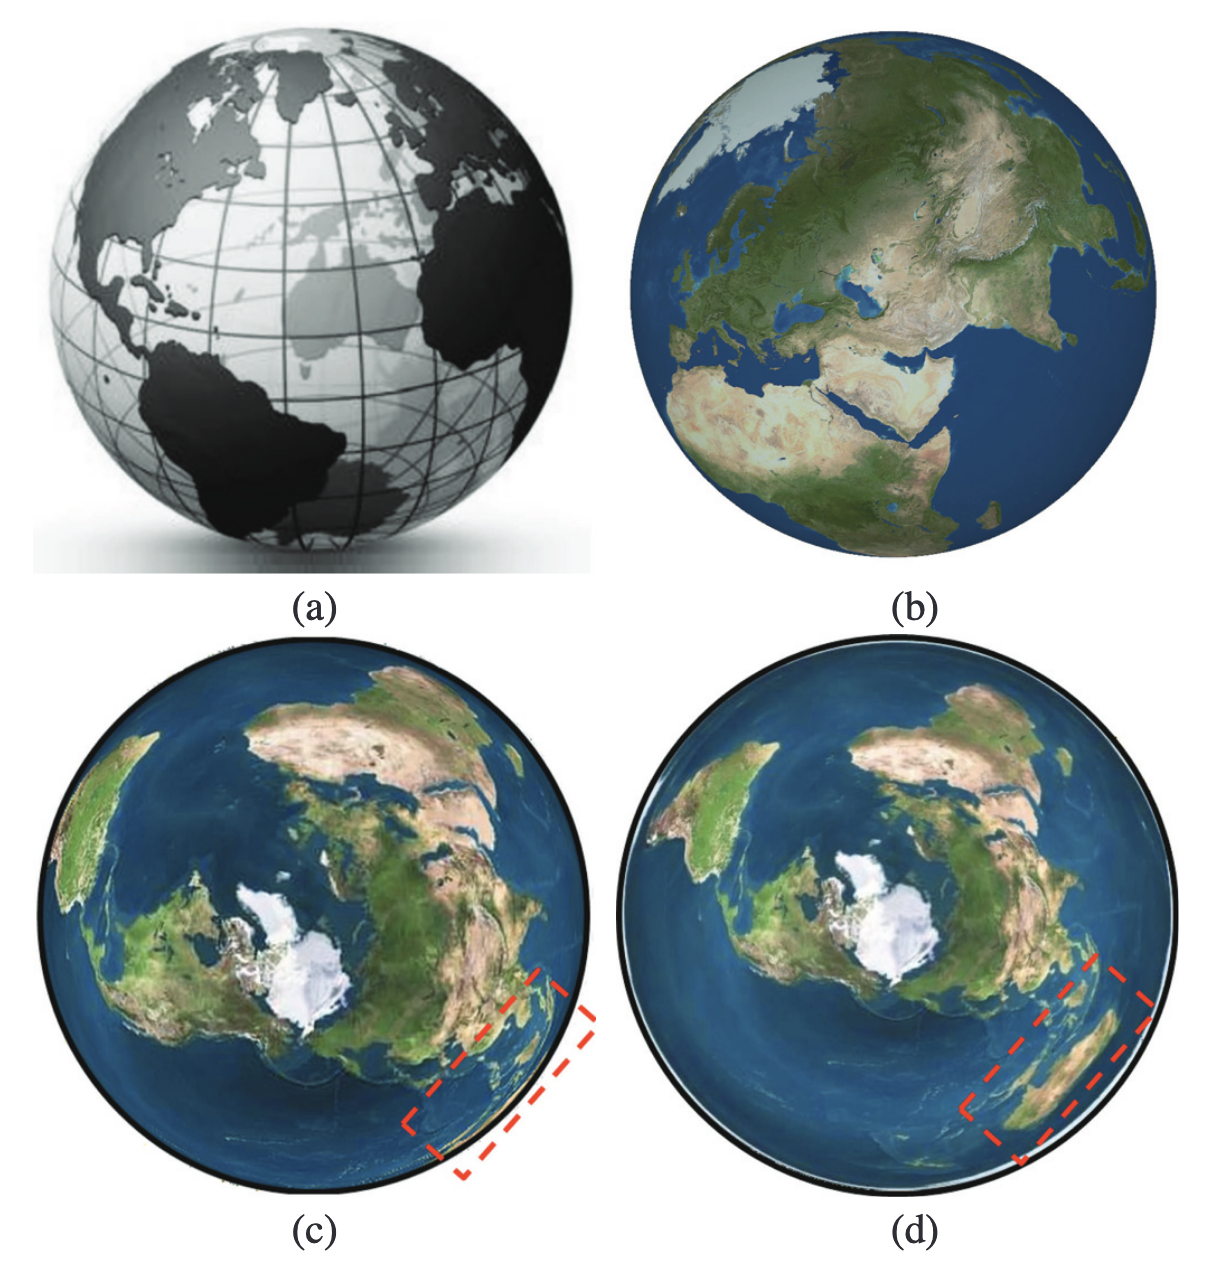
\includegraphics[width=\textwidth]{png/earth.png}
            \caption{
            (a) A 3D earth model. (b) Direct projection mapping with large information loss. 
            (c) Conformal mapping result with large area distortions. 
            (d) Area-preservation mapping result with accurate area preservation and 
            small angle distortion.}
        \end{minipage}
    \end{figure}
\end{frame}

\begin{frame}{Domain adaptation\footfullcite{courty_optimal_2017}}
    \footnotesize
    \vspace{-.8em}
    \begin{figure}
        \centering
        \captionsetup{font=scriptsize}
        \centering
        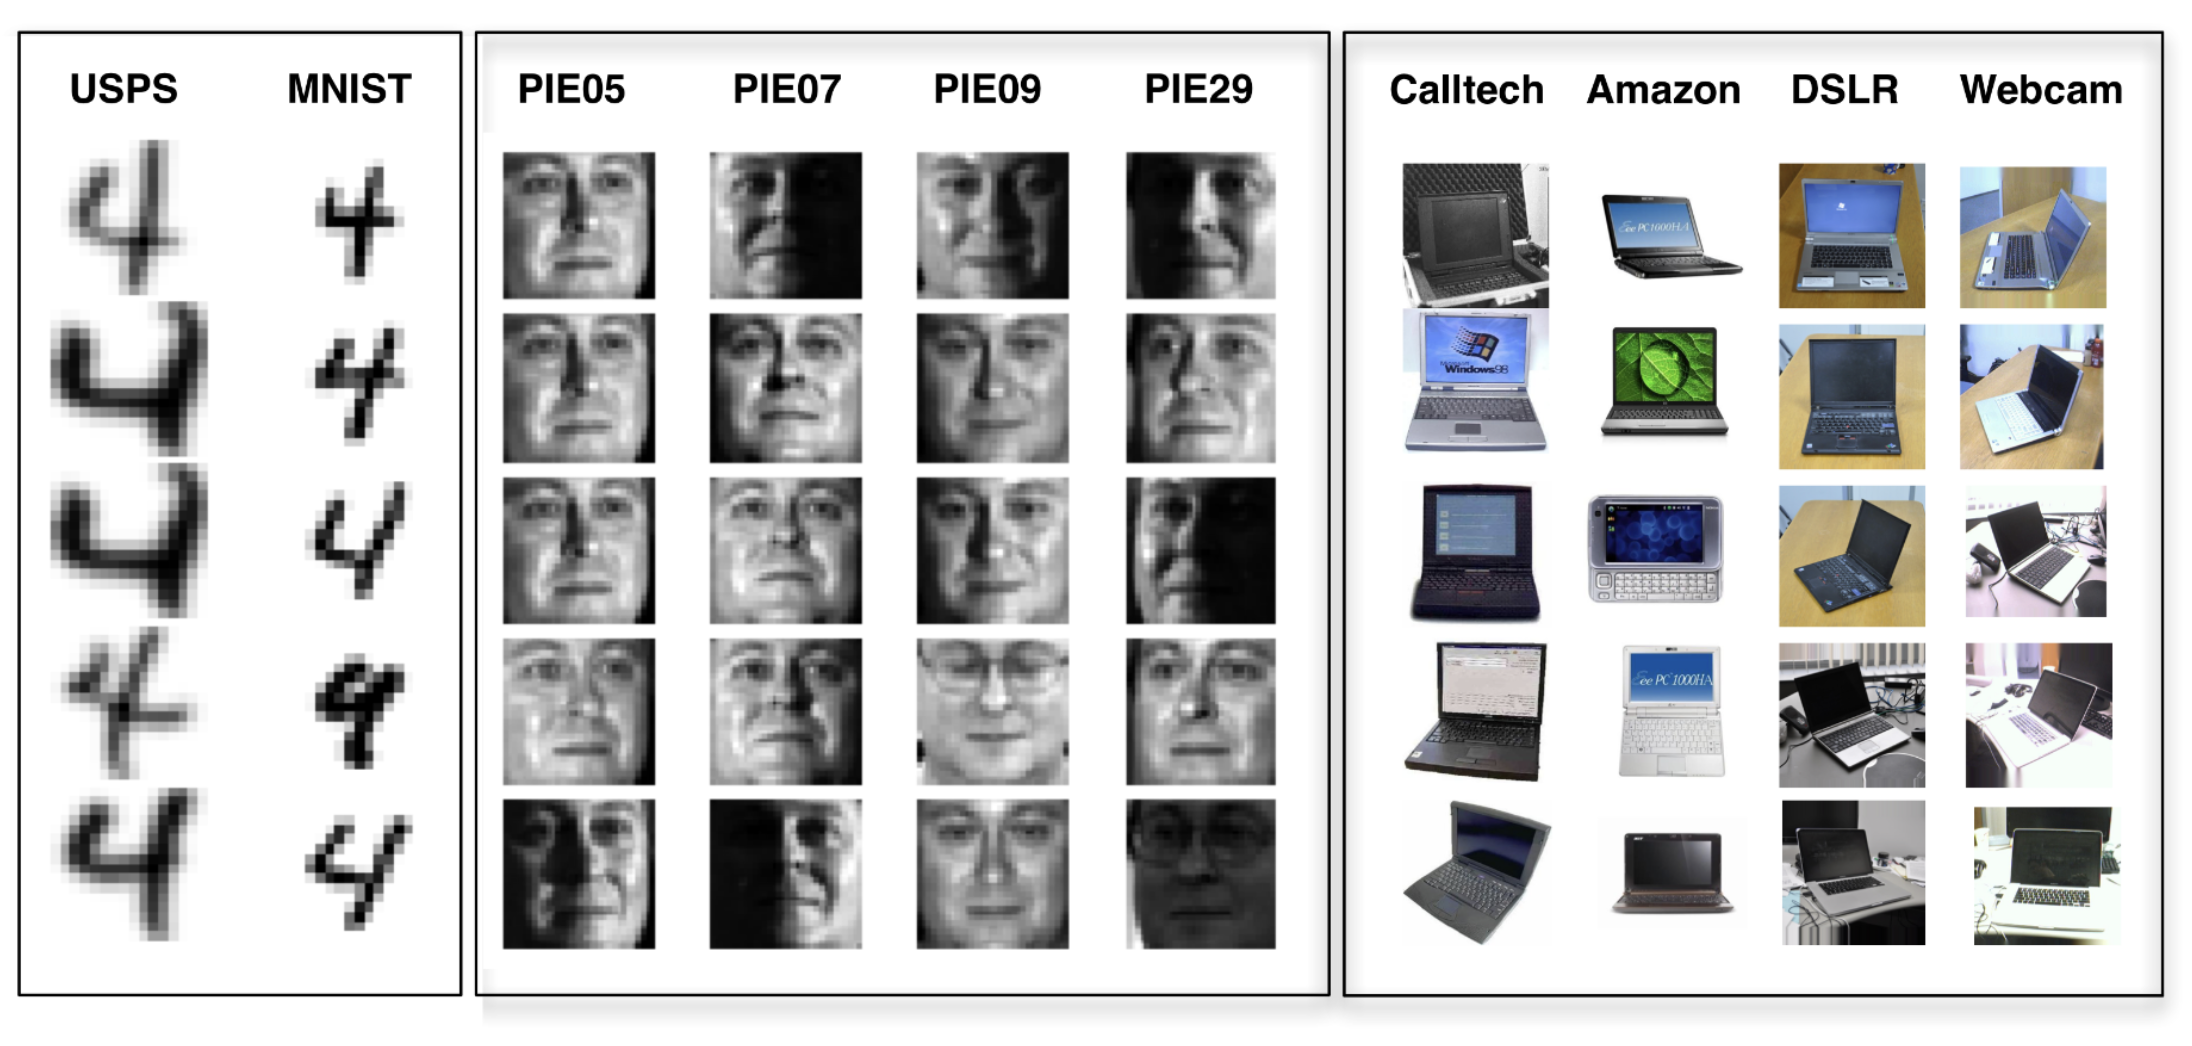
\includegraphics[width=0.65\textwidth]{png/domain-adapt-fig4.png}
        \vspace{-.8em}
        \caption{Examples of domain adaptation.}
    \end{figure}

    \vspace{-1.2em}
    \begin{figure}
        \centering
        \captionsetup{font=scriptsize}
        \centering
        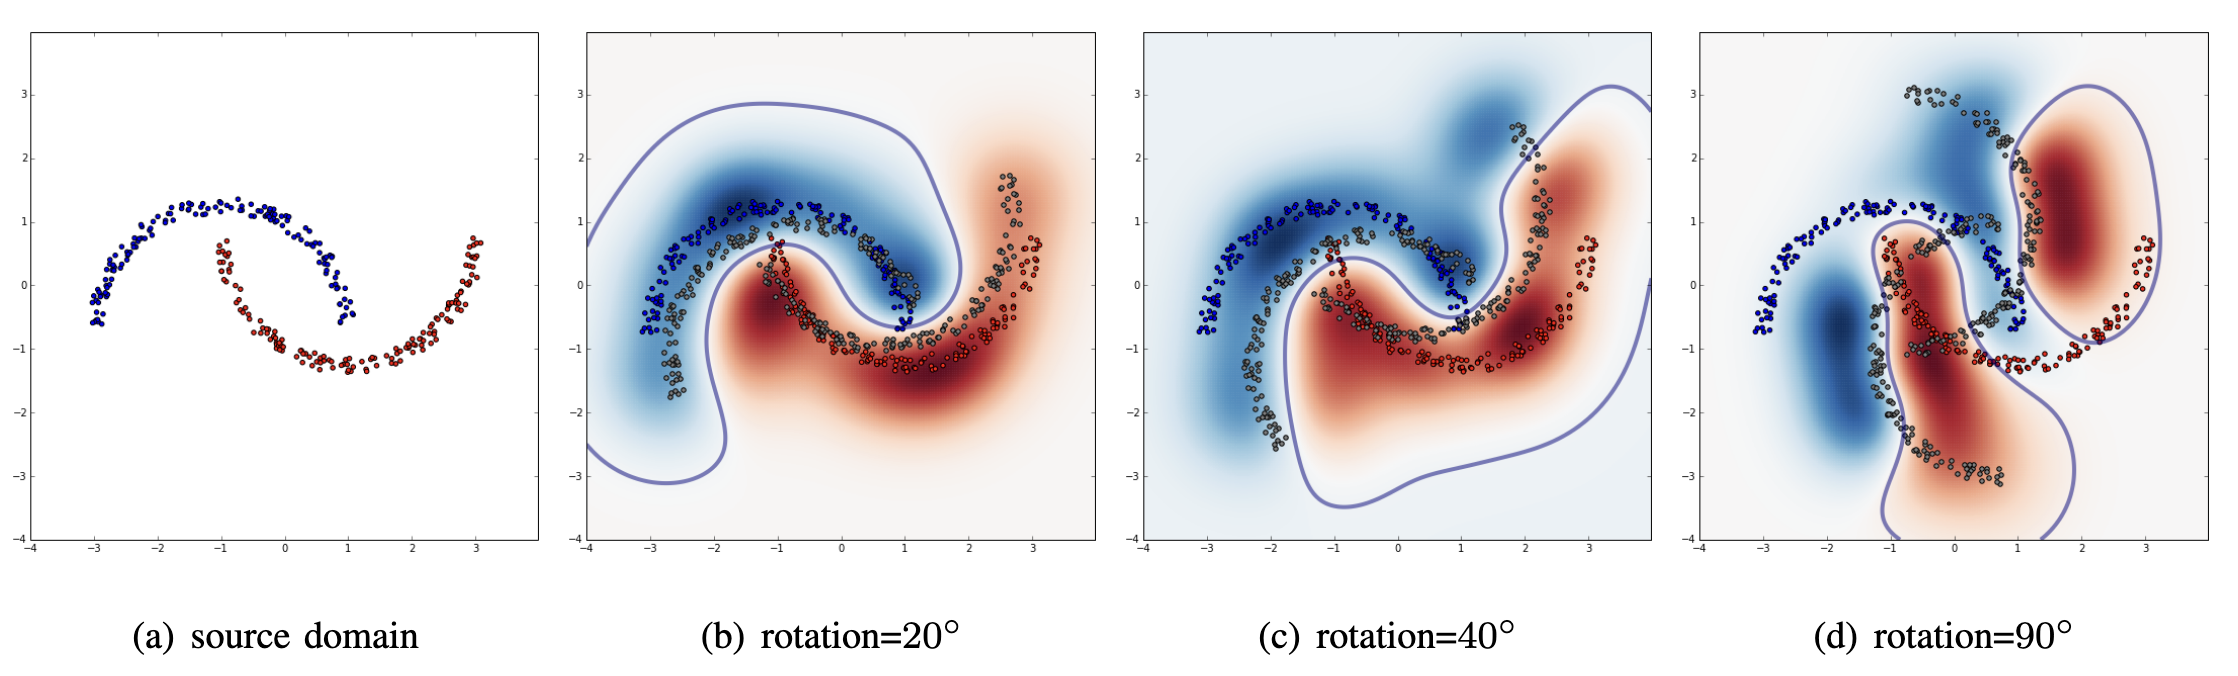
\includegraphics[width=0.85\textwidth]{png/domain-adapt-fig3.png}
        \vspace{-.8em}
        \caption{OT-based domain adaptation algorithm tested in a toy example.}
    \end{figure}
\end{frame}